\documentclass[10pt]{article}
% \usepackage[utf8]{vietnam}
\usepackage{vntex}
\usepackage{tikz}
\usepackage[left=3.00cm, right=2.00cm, top=2.00cm, bottom=2.00cm]{geometry}
\usepackage[unicode]{hyperref}
\usepackage{amsmath}
\usepackage{amssymb}
\usepackage{graphicx}
\usepackage{a4wide,amssymb,epsfig,latexsym,array,hhline,fancyhdr}
\usepackage[normalem]{ulem}
\usepackage[makeroom]{cancel}
\usepackage{amsmath}
\usepackage{amsthm}
\usepackage{multicol,longtable,amscd}
\usepackage{diagbox}
\usepackage{booktabs}
\usepackage{alltt}
\usepackage[framemethod=tikz]{mdframed}
\usepackage{caption,subcaption}
\usepackage[left=3.00cm, right=2.00cm, top=2.00cm, bottom=2.00cm]{geometry}
\usepackage{listings}
\usepackage{color}
\usepackage{lipsum}
\usepackage{setspace}
\usepackage{indentfirst}

\usetikzlibrary{decorations}
\usetikzlibrary{decorations.pathreplacing}
\usetikzlibrary{decorations.pathreplacing,calligraphy}
\setstretch{1}

\definecolor{dkgreen}{rgb}{0,0.6,0}
\definecolor{gray}{rgb}{0.5,0.5,0.5}
\definecolor{mauve}{rgb}{0.58,0,0.82}

\lstset{frame=tb,
  language=C++,
  aboveskip=3mm,
  belowskip=3mm,
  showstringspaces=false,
  columns=flexible,
  basicstyle={\small\ttfamily},
  numbers=none,
  numberstyle=\tiny\color{gray},
  keywordstyle=\color{purple},
  commentstyle=\color{dkgreen},
  stringstyle=\color{orange},
  breaklines=true,
  breakatwhitespace=true,
  tabsize=4
}

\title{CSES}
\author{Nguyễn Đức Huy}

\begin{document}
\maketitle
\tableofcontents
\newpage

\section{Two Knight}
\indent \url{https://cses.fi/problemset/task/1072}

Bài này có rất nhiều cách làm, dưới đây là 2 trong số đó
\begin{quote}
    \subsection*{DP}
    Gọi số cách đặt 2 con mã thỏa mãn trên bàn cờ $n \times n$ là $dp[n]$

    Trường hợp cơ bản: $dp[1] = 0$

    Ta tính $dp[n + 1]$ dựa trên $dp[n]$ như sau:

    \begin{center}
        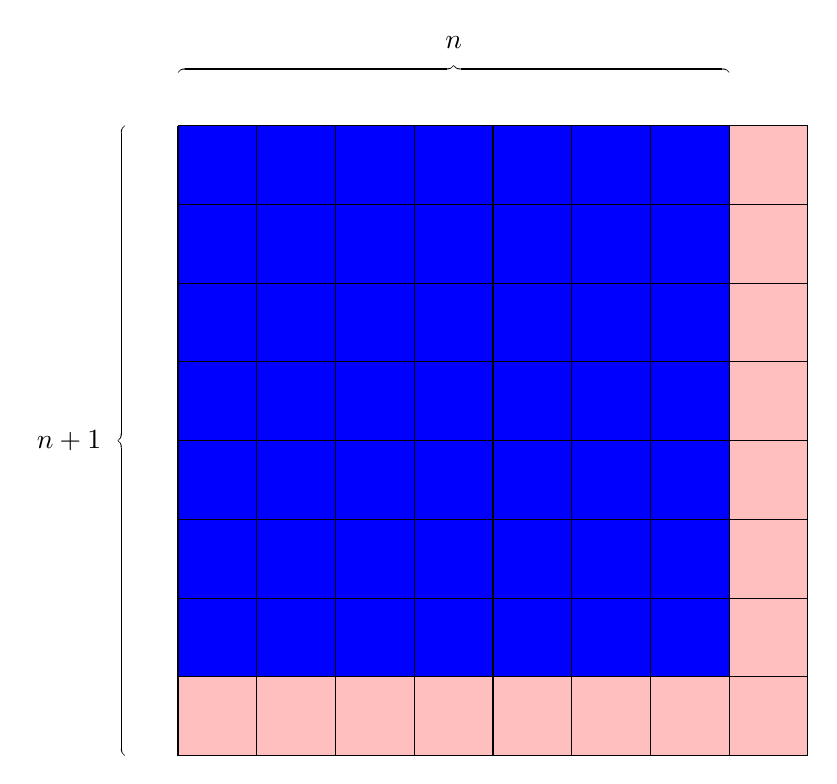
\begin{tikzpicture}

            \foreach \x in {0,1,2,3,4,5,6} {
                    \foreach \y in {1,2,3,4,5,6,7} {
                            \fill[blue] (\x,\y) rectangle (\x+1,\y+1);
                        }
                }

            \foreach \x in {0,1,2,3,4,5,6,7} {
                    \fill[pink] (\x,0) rectangle (\x+1,1);
                }

            \foreach \x in {1,2,3,4,5,6,7} {
                    \fill[pink] (7,\x) rectangle (8,\x+1);
                }

            \draw (0,0) grid (8,8);

            \draw [decorate, decoration = {calligraphic brace, raise=5pt}] (-0.5,0) --  (-0.5,8) node[pos=0.5,left=10pt,black]{$n+1$} ;
            \draw [decorate, decoration = {calligraphic brace, raise=5pt}] (0,8.5) --  (7,8.5) node[pos=0.5,above=10pt,black]{$n$} ;
        \end{tikzpicture}
    \end{center}
    Để đặt 2 con mã thỏa mãn lên bàn cờ $(n + 1) \times  (n + 1)$ thì có 3 cách
    \begin{enumerate}
        \item Cả 2 con ở vùng màu xanh $\Rightarrow dp[n]$
        \item Có 1 con ở vùng màu xanh và 1 con ở vùng màu hồng
        \item Cả 2 con ở vùng màu hồng
    \end{enumerate}

    Ta có công thức truy hồi:

    $ dp[n+1] = dp[n] + (((n - 1) * (n - 1) - 2) * 2 + ((n - 1) * (n - 1) - 3) * 2 + ((n - 1) * (n - 1) - 4) * (n - 1 - 4)) * 2 + ((n - 1) * (n - 1) - 2) + (2 * n - 1) * (n - 1) - 2 $

    Code mẫu:
    \begin{lstlisting}
        #include <bits/stdc++.h>
        using namespace std;

        int main()
        {
            long long int n;
            cin >> n;
            long long int dp = 0;
            long long int c = 1;

            while (c <= n)
            {
                c++;
                cout << dp << endl;
                dp = dp + (((c - 1) * (c - 1)- 2) * 2 + ((c - 1) * (c - 1) - 3) * 2 + ((c - 1) * (c - 1) - 4) * (c -1 - 4)) * 2 + ((c - 1) * (c - 1) - 2) + (2 * c - 1) * (c - 1) - 2;
            }
        }
    \end{lstlisting}

    \subsection*{Math}
    2 quân mã có thể tấn công nhau thì nó phải ở trong hình chữ nhật $2 \times 3$ hoặc $3 \times 2$, mỗi hình chữ nhật như thế sẽ cho 2 cách đặt con mã có thể tấn công nhau. Nghĩa là có tất cả $2 \times ((n - 1)(n - 2) + (n - 2)(n - 1))$ cách

    Vậy :D để 2 con mã không tấn công nhau thì có $C^2_{n^2} - 2 \times ((n - 1)(n - 2) + (n - 2)(n - 1))$ cách

    Code mẫu:
    \begin{lstlisting}
        #include <bits/stdc++.h>
        using namespace std;
        int main()
        {
            long long int n;
            cin >> n;
            for (long long int i = 1; i <= n; i++)
            cout    << (i * i) * (i * i - 1) / 2 - 4 * ((i - 1) * (i - 2))
                    << endl;
        }
    \end{lstlisting}
\end{quote}
\newpage
\section{Two Sets}
\url{https://cses.fi/problemset/task/1092}

Trước hết, ta phân tích một chút.

Tổng $1 + 2 + 3 + \ldots + n = \frac{n(n+1)}{2}$. Để chia tổng này thành 2 tập có tổng bằng nhau thì tổng này phải chẵn, nghĩa là $\frac{n(n+1)}{2}$ chia hết cho 2 $\Rightarrow n(n + 1)$ chia hết cho 4

$\Rightarrow n$ chia hết cho 4 hoặc $n$ chia 4 dư 3

Với $n$ chia hết cho 4, ta chia tổng $n$ số thành $\frac{n}{2}$ cặp đầu cuối có tổng bằng nhau, vì $n$ chia hết cho 4 nên $\frac{n}{2}$ chẵn, khi đó, ta chỉ cần chọn bừa $\frac{n}{4}$ cặp đầu cuỗi cho vào tập thứ nhất và $\frac{n}{4}$ cặp còn lại cho vào tập thứ 2.

Với $n$ chia 4 dư 3, ta xếp số $1$ và $2$ vào tập thứ nhất, số $3$ vào tập thứ 2. Với những số còn lại, tương tự trường hợp trên.

Code mẫu:
\begin{lstlisting}
    #include <bits/stdc++.h>
    using namespace std;

    vector<int> a, b;

    void solve(int l, int r)
    {
        if (r < l)
            return;

        a.push_back(l);
        a.push_back(r);
        b.push_back(l + 1);
        b.push_back(r - 1);

        solve(l + 2, r - 2);
    }
    int main()
    {
        int n;
        cin >> n;
        if (n % 4 == 1 || n % 4 == 2)
        {
            cout << "NO";
            return 0;
        }
        if (n % 4 == 3)
        {
            a.push_back(1);
            a.push_back(2);
            b.push_back(3);
        }

        solve(n % 4 + 1, n);

        cout << "YES" << endl;
        cout << a.size() << endl;
        for (int i = 0; i < a.size(); i++)
            cout << a[i] << (i == a.size() - 1 ? "\n" : " ");
        cout << b.size() << endl;
        for (int i = 0; i < b.size(); i++)
            cout << b[i] << (i == b.size() - 1 ? "\n" : " ");
    }
\end{lstlisting}
\end{document}